\section{Background on Low-Rank fODF Tensor Approximation}\label{sec:background}
Earliest approaches for dMRI tractography used the diffusion tensor model
\cite{Mori:1999}, and were therefore limited to a single dominant fiber orientation
per voxel. However, most white matter voxels contain more than one fiber bundle \cite{Jeurissen:2012}, and it has been shown
that accounting for these more complex fiber geometries greatly improves dMRI
tractography \cite{Neher:2015}.

Our work builds on a previously described low-rank approximation of fODF tensors to infer multiple fiber orientations per voxel \cite{lowrank,Ankele:CARS2017}. It first obtains a symmetric \added{fourth}-order tensor representation $\mathcal{T}$ of the fiber orientation distribution function (fODF) via constrained spherical deconvolution, which amounts to solving the linear least squares problem 
\begin{align}
	\argmin_{\mathcal{T}} \| M \mathcal{T} - S \|^2,
	\label{eq:sd-min}
\end{align}
where 
$M$ denotes a convolution matrix that is based on the dMRI response from a
single fiber compartment, vector $S$ contains all dMRI measurements in a given
voxel. A set of $r$ fiber directions is then estimated as unit vectors
$\mathbf{v}_i \in \mathbb{R}^3$ with volume fractions $\lambda_i$ for $i \in
\left\{ 1 , \dots , r \right\}$ via a rank-$r$
approximation 
\begin{align}
	\mathcal{T}^{\left( r \right)} = \sum_{i=1}^r \lambda_i \mathbf{v}_i
	\otimes \mathbf{v}_i \otimes \mathbf{v}_i \otimes \mathbf{v}_i,
	\label{eq:low-rank}
\end{align}
where $\otimes$ denotes the
outer product. The approximation is formalized as
\[ \argmin_{\lambda_1, \dots , \lambda_r , \mathbf{v}_1, \dots , \mathbf{v}_r}
\| \mathcal{T} - \mathcal{T}^{\left( r \right)} \|_F, \]
where $\| \cdot \|_F$ denotes the Frobenius norm.

\begin{figure*}[t]
	\centering
	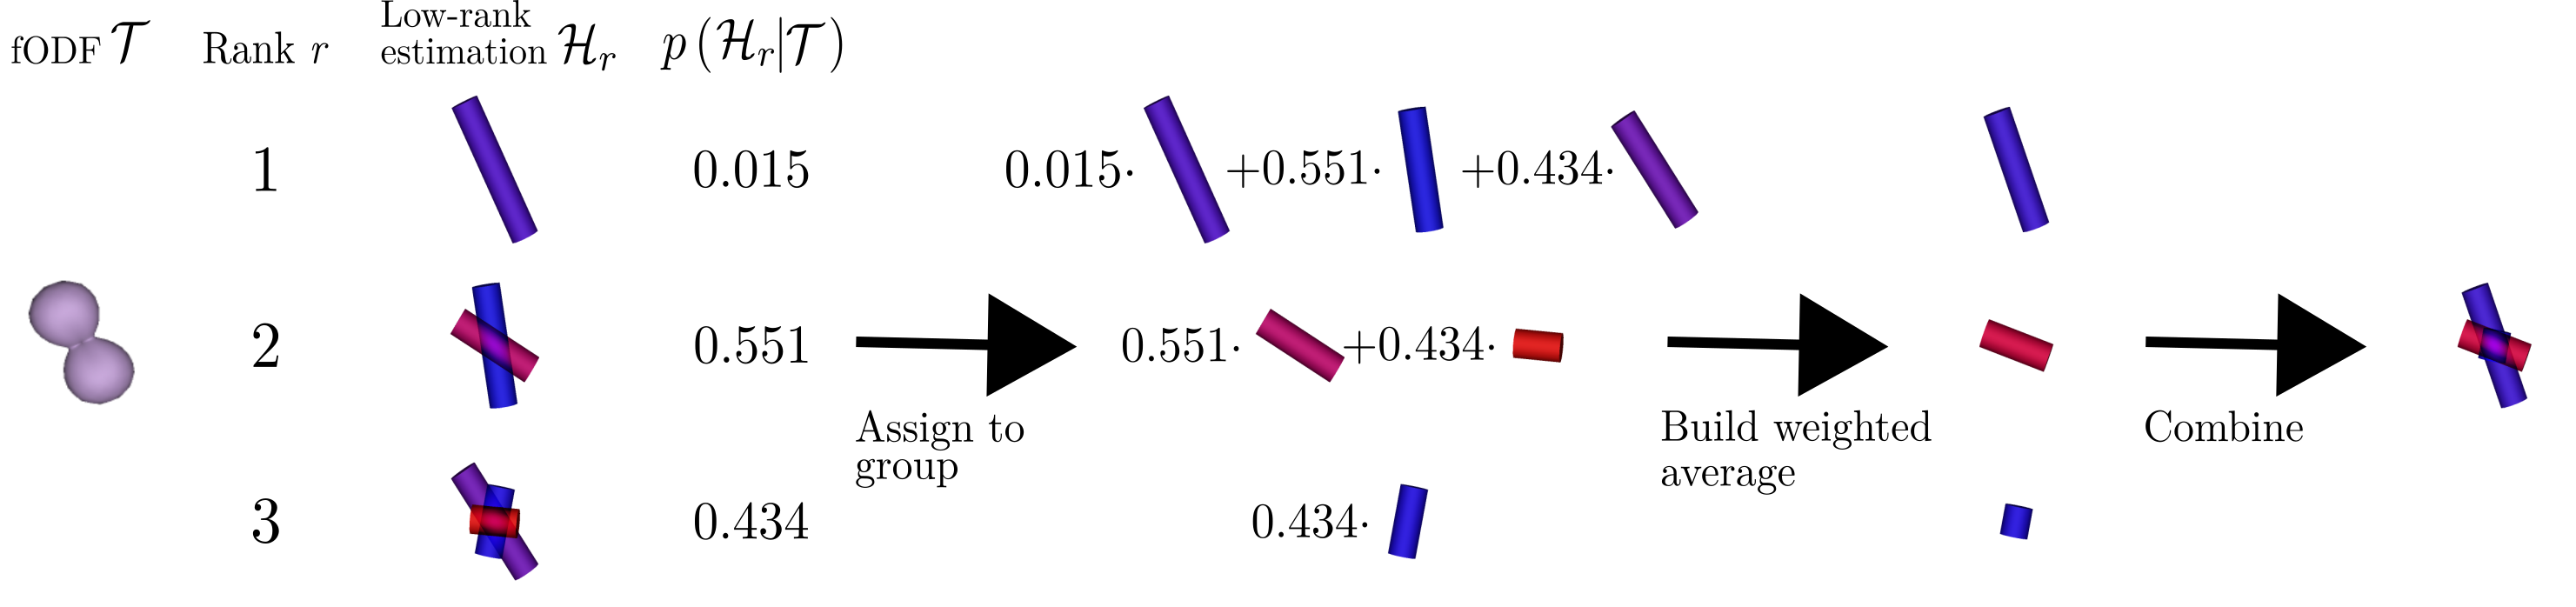
\includegraphics[width=\linewidth]{base_overview_scheme}
	\caption{\added{Illustration of our model averaging strategy. For a given fODF $\mathcal{T}$, low-rank approximations with ranks $r \in \left\{ 1,2 , 3 \right\}$ are computed. The resulting directions are clustered, and a weighted average is taken within each group, with weights given by the posterior model probabilities $p \left( \mathcal{H}_r \mid \mathcal{T} \right)$ from a Bayesian framework. This results in a combined model in which secondary and tertiary fibers fade in and out smoothly in regions of model uncertainty, rather than vanishing abruptly, as when selecting the most likely model.}}
	\label{fig:base_overview}
\end{figure*}

These steps represent a refinement of a more traditional approach to spherical deconvolution, which is based on spherical harmonics, a soft non-negativity constraint, and taking local fODF maxima as fiber directions \cite{TOURNIER20071459}. It has been demonstrated that replacing peak extraction with low-rank approximation reduces angular errors, and increases angular resolution, even when replacing the more traditional spherical harmonics of degree eight with fourth-order tensors, which have much fewer degrees of freedom, and greatly improve the conditioning of the least squares problem \cite{Ankele:CARS2017}.

The non-negativity constraint in spherical deconvolution is justified by
the fact that the fODF represents the fiber fraction in any given
direction, which must be non-negative. In the tensorial framework, it is implemented by imposing a positive semi-definiteness constraint on $\mathcal{T}$, which also ensures that all $\lambda_i$ in Eq.~(\ref{eq:low-rank}) will be non-negative \cite{Ankele:CARS2017}. 

% I don't agree with the following.
% Our original 2008 paper used simulated data with a noise term, the 2017
% paper resampled noisy data. I would argue that both types of experiment
% provide insight on how strongly noise affects our estimates.
%Neither CSD nor the low-rank approximation is resistant against
%measurement noise. The resistance against noise has not been evaluated for the
%CSD with H-psd and low-rank $r$ approximation. From a theoretical point of view
%the unregularized low-rank $r$ approximation should be very sensitive for small
%changes in the fODFs.

%%% Local Variables:
%%% mode: latex
%%% TeX-master: "../main"
%%% End:
